\documentclass[3p,fleqn]{elsarticle}
\journal{Computer Physics Communications}

%%%%%%%%%%%%%%%%%%%%%%%%%%%%%%%%%%%%%%%%%%%%%%%%%%%%%%%%%%%%%%%%%%%%%%%%%%%%%%%%
\usepackage[charter]{mathdesign}
\usepackage[T1]{fontenc}         % Use T1 encoding instead of OT1
\usepackage[utf8]{inputenc}      % Use UTF8 input encoding
\usepackage{microtype}           % Improve typography
\usepackage{booktabs}            % Publication quality tables
\usepackage{amsmath}
\usepackage{float}
\usepackage{algorithm}
\usepackage{algorithmicx}
\usepackage{algpseudocode}
\usepackage[binary-units=true,exponent-product=\cdot]{siunitx}

\usepackage[colorlinks,breaklinks]{hyperref}

% Captions for figures and tables
\usepackage[labelfont=bf]{caption}
\captionsetup[figure]{labelsep=period, name=Fig.}
\captionsetup[table]{labelsep=newline}
\usepackage{subcaption}

% Set correct abbreviations
\def\equationautorefname{Eq.}
\def\figureautorefname{Fig.}
\def\algorithmautorefname{Algorithm}
\DeclareMathOperator\expint{E_1}

\newcommand{\tmax}{T_{\mathrm{M}}}
\newcommand{\ef}{E_{\mathrm{F}}}
\newcommand{\efl}{E_{\mathrm{F}}^{\mathrm{L}}}
\newcommand{\efh}{E_{\mathrm{F}}^{\mathrm{H}}}

%%%%%%%%%%%%%%%%%%%%%%%%%%%%%%%%%%%%%%%%%%%%%%%%%%%%%%%%%%%%%%%%%%%%%%%%%%%%%%%%
\begin{document}

\title{An algorithm for generating random variates from the Madland-Nix fission
  energy spectrum}

\author{Paul K. Romano\corref{cor1}}
\ead{paul.romano@unnpp.gov}
\cortext[cor1]{Corresponding author. Tel.: +1 518 395 4010.}

\address{Bechtel Marine Propulsion Corporation, Knolls Atomic Power
  Laboratory \\ P.O. Box 1072, Schenectady, NY 12301, United States}


\begin{abstract}
  An algorithm for generating random variates from the Madland-Nix fission
  energy spectrum assuming a constant compound nucleus cross section is given
  based on physics considerations. A program was written to generate variates
  using the algorithm developed, and it was shown that the generated variates
  match the probability density function. This algorithm can be used by
  Monte Carlo particle transport codes to sample secondary energies for neutrons
  born from fission when the underlying data is given as parameters to a
  Madland-Nix energy spectrum.
\end{abstract}

\begin{keyword}
  Madland-Nix, fission, spectrum, random variate, algorithm
\end{keyword}

\maketitle

%%%%%%%%%%%%%%%%%%%%%%%%%%%%%%%%%%%%%%%%%%%%%%%%%%%%%%%%%%%%%%%%%%%%%%%%%%%%%%%%
\section{Introduction}

Evaluated nuclear data used for nuclear technology applications are commonly
stored in a format called ENDF-6~\cite{bnl-trkov-2012}. This format covers a
wide variety of data including cross sections for neutron- and photon-induced
reactions, radioactive decay data, fission product yields, thermal neutron
scattering functions, and variances/covariances of these data. One important
category of data in ENDF is secondary angle and energy distributions for
particles emerging from nuclear reactions. These secondary distributions can
assume a number of different representations. In this paper, we will focus on
one particular representation of a secondary energy distribution in ENDF called
the Madland-Nix energy spectrum\footnote{Throughout this paper, the terms
  \textit{energy distribution} and \textit{energy spectrum} are used
  interchangeably.}.

Simulations of systems containing fissionable materials can be particularly
sensitive to the energy distributions of neutrons born from fission. Thus, it is
important that the evaluated data for these energy distributions faithfully
represent the experimental data. One way of achieving highly accurate data is to
store the data in tabulated form along with a specification for how the data are
to be interpolated between tabulated values. However, this can result in a very
large dataset. Nuclear reaction theory can give insights into the expected
analytical forms for fundamental data. Therefore, it is common for evaluators to
fit the experimental data to analytical forms which enables them to store only
the parameters of the analytical function rather than a large tabulated dataset.

For fission reactions, several analytical forms exist to describe the energy
distribution of outgoing neutrons. Two simple forms are the Maxwellian energy
spectrum and the Watt energy spectrum~\cite{physrev-watt-1952}. The Maxwellian
and Watt energy spectra have the advantage that their probability density
functions are relatively simple; there are numerous algorithms for generating
random variates from these distributions. This, in turn, means that Monte Carlo
particle transport codes need only store the parameters for these
distributions. For the Maxwellian spectrum, the distribution is specified by a
single parameter; for the Watt spectrum, it is fully defined by two parameters.

While the Maxwellian and Watt distributions give reasonable fits to fission
energy spectra for many nuclides, both distributions neglect several important
physical effects. An improvement on these spectra was made by Madland and Nix
\cite{nse-madland-1982} by accounting for the distribution of fission-fragment
residual nuclear temperature and the energy dependence of the cross section for
the inverse process of compound nucleus formation. The result is known as the
Madland-Nix energy spectrum, also sometimes referred to as the Los Alamos
model.

Due to the success of the Madland-Nix theory in predicting and fitting
experimental data for prompt fission neutron energy spectra, an option is
available in the ENDF-6 format to represent energy spectra by specifying
parameters to the Madland-Nix density function. In the ENDF/B-VII.1 data
library~\cite{nds-chadwick-2011}, $^{241}$Am and $^{243}$Am have fission neutron
energy distributions that use the Madland-Nix representation.

As will be shown in \autoref{sec:density}, the density function for the
Madland-Nix spectrum consists of a combination of exponential integrals and
incomplete gamma functions. As such, the analytical form does not lend itself
to any straightforward sampling scheme; the current norm is for nuclear data
processing codes, such as NJOY~\cite{lanl-macfarlane-2012} and
NDEX~\cite{snamc-griesheimer-2013}, to convert these spectra to tabulated
density functions before writing them to data files used for Monte Carlo
simulations.

In this paper, an algorithm to generate random variates from the Madland-Nix
density function as specified by the ENDF-6 format is given. This algorithm
will 1) enable nuclear data processing codes to pass evaluated data for such
energy spectra directly to the formats used by Monte Carlo particle transport
codes and 2) enable Monte Carlo codes to sample the energy distribution given
the parameters for the Madland-Nix density function.

%%%%%%%%%%%%%%%%%%%%%%%%%%%%%%%%%%%%%%%%%%%%%%%%%%%%%%%%%%%%%%%%%%%%%%%%%%%%%%%%
\section{Density Function}
\label{sec:density}

It is instructive to first go through a derivation of the Madland-Nix
density function as the details of the derivation will be useful for
developing a sampling algorithm. Madland and Nix's
approach~\cite{nse-madland-1982} was to use evaporation theory to determine the
neutron energy spectrum in the center-of-mass system and then to transform it to
the laboratory system. In the fission process, the target nuclide splits into
two fragments each of which has residual excitation energy. The fragments may
subsequently de-excite by emitting neutrons. Under the assumption that the
neutron energy is small compared to the excitation energy less the separation
energy of the neutron, the center-of-mass energy spectrum corresponding to a
fixed nuclear temperature $T$ can be shown to be~\cite{physrev-weisskopf-1937}
\begin{equation}
  \phi(\epsilon) = \frac{\epsilon}{T^2} e^{-\epsilon/T}
  \label{eq:evaporation}
\end{equation}
where $\epsilon$ is the center-of-mass neutron energy. This spectrum is referred
to as an \textit{evaporation spectrum} since the process by which neutrons are
emitted from the excited nucleus is analogous to thermodynamic evaporation
processes. However, the nuclear temperature, which is related to the excitation
energy, is not fixed but rather assumes a distribution of its
own. Terrell~\cite{physrev-terrell-1959} observed that the distribution of
fission-fragment residual nuclear temperature can be approximated by a
triangular distribution as
\begin{equation}
  P(T) = \begin{cases} 2T/\tmax^2, & T \le \tmax \\ 0, & T > \tmax \end{cases}
  \label{eq:triangle}
\end{equation}
where $\tmax$ is the maximum nuclear temperature. Thus, the center-of-mass energy
distribution of neutrons emitted from fission fragments is obtained by averaging
\autoref{eq:evaporation} over the temperature distribution in \autoref{eq:triangle}:
\begin{equation}
  \Phi(\epsilon) = \int_0^\infty \phi(\epsilon) P(T) dT =
  \frac{2\epsilon}{\tmax^2} \expint ( \epsilon/\tmax )
  \label{eq:com}
\end{equation}
where
\begin{equation*}
  \expint(x) = \int_x^\infty \frac{e^{-u}}{u} du
\end{equation*}
is related to the exponential integral. To obtain the distribution of neutrons
in the laboratory system, we must transform the energies in the center-of-mass
system. Under the assumption that the neutron is emitted isotropically from a
fission fragment with average kinetic energy per nucleon $\ef$, the distribution
function in the laboratory system can be shown to be~\cite{physrev-terrell-1959}
\begin{equation}
  g(E,\ef) = \frac{1}{4\sqrt{\ef}} \int_{\left( \sqrt{E} - \sqrt{\ef}
    \right)^2}^{\left( \sqrt{E} + \sqrt{\ef} \right)^2}
  \frac{\Phi(\epsilon)}{\sqrt{\epsilon}} d\epsilon.
  \label{eq:com-to-lab}
\end{equation}
Inserting \autoref{eq:com} into \autoref{eq:com-to-lab} and evaluating the integral
analytically yields the energy distribution in the laboratory system:
\begin{equation}
  g(E,\ef) = \frac{1}{3\sqrt{\ef \tmax}} \bigg [ u_2^{3/2} \expint (u_2) -
    u_1^{3/2} \expint (u_1) + \gamma \left( \frac{3}{2}, u_2 \right ) -
    \gamma \left( \frac{3}{2}, u_1 \right) \bigg ]
\end{equation}
where $u_1 = \left ( \sqrt{E} - \sqrt{\ef} \right )^2/\tmax$, $u_2 = \left (
\sqrt{E} + \sqrt{\ef} \right)^2/\tmax$, and $\gamma(a,x)$ is the lower incomplete
gamma function defined as
\begin{equation*}
  \gamma(a,x) = \int_0^x u^{a-1} e^{-u} du.
\end{equation*}
Since the laboratory energy distribution depends on $\ef$, it will be different
for light and heavy fragments given that a heavier fragment has lower velocity
and hence lower average kinetic energy. Madland and Nix argue that the number of
neutrons emitted from the light and heavy fission fragments is approximately
equal in the vicinity of the average fragments; thus, the energy spectrum
accounting for neutrons emitted from both light and heavy fragments is simply an
average of the two. Denoting $\efl$ and $\efh$ the average kinetic energy per
nucleon of the light and heavy fragments, respectively, the final form of the
Madland-Nix energy spectrum is
\begin{equation}
  \label{eq:spectrum}
  f(E) = \frac{1}{2} \left [ g(E, \efl) + g(E, \efh) \right ].
\end{equation}
This equation is equivalent to the representation in the ENDF-6
format~\cite{bnl-trkov-2012} under File 5, LF=12.

Strictly speaking, \autoref{eq:spectrum} still ignores the dependence of the
center-of-mass energy spectrum on the cross section for the inverse process of
compound nucleus formation that Madland and Nix had accounted for. However, the
ENDF-6 format only includes the representation assuming a constant compound
nucleus cross section. If an evaluator did wish to take into account the
compound nucleus cross section, the evaluated data would simply have to be given
in tabulated form.

%%%%%%%%%%%%%%%%%%%%%%%%%%%%%%%%%%%%%%%%%%%%%%%%%%%%%%%%%%%%%%%%%%%%%%%%%%%%%%%%
\section{Sampling Algorithm}

While the density function in \autoref{eq:spectrum} does not naturally lend
itself to standard techniques for non-uniform random variate generation, an
algorithm can be developed based on the physical processes outlined in the
derivation of the spectrum. The center-of-mass energy spectrum was given as the
convolution of an evaporation spectrum with a triangular distribution for the
residual nuclear temperature. Thus, it can be sampled by first sampling a
temperature from the triangular temperature distribution and then using the
sampled temperature as the parameter in an evaporation spectrum. The cumulative
distribution function for temperature is $F(T) = T^2/\tmax^2$ for $T \le
\tmax$. Inverting this cumulative distribution allows us to generate random
variates $T = \tmax \sqrt{\xi_1}$ where $\xi_1$ is a random variate sampled from
the uniform distribution on $[0,1]$. Note that in the ENDF-6 format, $\tmax$ is
given as a tabulated function of incident neutron energy. An algorithm for
sampling the evaporation spectrum is given by rule C45 from the Monte Carlo
Sampler~\cite{lanl-everett-1983}:
\begin{equation*}
  \epsilon = -T \log (\xi_2 \xi_3)
\end{equation*}
where $\xi_2$ and $\xi_3$ are also uniformly-distributed random variates. The
center-of-mass energy must then be transformed to the laboratory system using an
expression from Terrell~\cite{physrev-terrell-1959}:
\begin{equation}
  E = \epsilon + \ef + 2\mu \sqrt{\ef \epsilon}
  \label{eq:com-to-lab2}
\end{equation}
where $\mu$ is the cosine of the angle of emission in the center-of-mass
system. It is well known that the cosine of an isotropic angular distribution
is uniformly distributed on $[-1,1]$. Thus, it can be sampled as $\mu = 2\xi_4
- 1$. Finally, we must use \autoref{eq:com-to-lab2} half of the time with
$\efl$ and half of the time with $\efh$ to achieve a distribution that is the
average of the light fragment and heavy fragment distribution. This can be done
easily by sampling a uniform random variate, $\xi_5$, checking whether it is
less than one-half, and if so using $\efl$ in \autoref{eq:com-to-lab2}.

Combining all the steps above, a summary of the algorithm is given in
\autoref{alg:madland-nix}. Despite the probability density function of the
Madland-Nix spectrum being quite complex, the algorithm presented here requires
no rejections, no evaluations of special functions, and only five uniform
variates.
\begin{algorithm}
  \caption{Random variate generation for the Madland-Nix fission energy spectrum
    assuming a constant compound nucleus cross section.}
  \label{alg:madland-nix}
  \begin{algorithmic}[1]
    \State Determine $\tmax$ as function of incident neutron energy
    \State $T \gets \tmax \sqrt{\xi_1}$
    \State $\epsilon \gets - T \log(\xi_2 \xi_3)$
    \State $\mu \gets 2\xi_4 - 1$
    \If{$\xi_5 < 1/2$}
      \State $E \gets \epsilon + \efl + 2\mu \sqrt{\efl \epsilon}$
    \Else
      \State $E \gets \epsilon + \efh + 2\mu \sqrt{\efh \epsilon}$
    \EndIf
  \end{algorithmic}
\end{algorithm}

It is worth noting that the same procedure used to develop the algorithm for the
Madland-Nix fission spectrum can also be used to derive a direct sampling scheme
for the Watt fission spectrum~\cite{lanl-brown-2005} that is used in several
Monte Carlo particle transport codes~\cite{snamc-griesheimer-2013,
  ane-romano-2013} but for which no explanation in the open literature has been
found. Physically, the Watt spectrum represents a Maxwellian spectrum in the
center-of-mass system that has been transformed to the laboratory system. If we
take a Maxwellian spectrum
\begin{equation*}
  \Phi(\epsilon) = \frac{2}{\sqrt{\pi T}} \sqrt{\epsilon} e^{-\epsilon/T},
\end{equation*}
insert it in \autoref{eq:com-to-lab}, and evaluate the integral, we obtain
\begin{equation}
  W(E) = \frac{e^{-\ef/T}}{\sqrt{\pi \ef T}} e^{-E/T} \sinh \sqrt{\frac{4\ef
      E}{T^2}}.
  \label{eq:watt1}
\end{equation}
The Watt spectrum is usually characterized by two parameters $a$ and $b$ as
\begin{equation}
  W(E) = \frac{2e^{-ab/4}}{\sqrt{\pi a^3 b}} e^{-E/a} \sinh \sqrt{bE}.
  \label{eq:watt2}
\end{equation}
Comparing \autoref{eq:watt1} and \autoref{eq:watt2}, we can relate the Watt
parameters to $\ef$ and $T$:
\begin{align*}
  a &= T \\
  b &= \frac{4\ef}{T^2}.
\end{align*}
Thus, the fragment kinetic energy per nucleon can be expressed as $\ef =
a^2b/4$. Substituting this expression into into \autoref{eq:com-to-lab2} gives us
the direct sampling scheme in~\cite{lanl-brown-2005}:
\begin{equation*}
  E = \epsilon + \frac{a^2b}{4} + \mu \sqrt{a^2 b \epsilon}
\end{equation*}
where $\epsilon$ is sampled from a Maxwellian spectrum.

%%%%%%%%%%%%%%%%%%%%%%%%%%%%%%%%%%%%%%%%%%%%%%%%%%%%%%%%%%%%%%%%%%%%%%%%%%%%%%%%
\section{Results}

In order to compare the speed and accuracy of the proposed algorithm, a program
was written in Julia~\cite{arxiv-bezanson-2012} to generate variates using
\autoref{alg:madland-nix} as well as the traditional algorithm used by Monte
Carlo neutron transport codes (a search on the tabulated cumulative
distribution function). For \autoref{alg:madland-nix}, variates are generated
using the $\tmax$, $\efl$, and $\efh$ parameters from the ENDF file. Values of
$\tmax$ corresponding to energies between those tabulated are determined using
the interpolation scheme specified in the ENDF file. For the traditional
algorithm, the ENDF file first needs to be processed using NJOY, resulting in
an ACE file that contains a tabulated probability density function (pdf) and
cumulative distribution function (cdf) at each incoming neutron energy for
which $\tmax$ is tabulated. However, since the tabulated distributions are only
given at specific incident energies, unit base
interpolation~\cite{nse-doyas-1972} is used to generate variates as an
approximation. Thus, the traditional algorithm is exact only at the tabulated
incident energies.

Random variates were generated for the ENDF/B-VII.1 $^{241}$Am fission spectrum
at two incident neutron energies. The first energy, $\SI{1e-5}{\electronvolt}$,
was chosen to correspond to an incident energy at which $\tmax$ was
tabulated. Based on the discussion above, both \autoref{alg:madland-nix} and
the traditional algorithm should be exact.  \autoref{fig:point} shows the
observed distribution of 10 million variates produced by each algorithm
compared to the analytical form given in \autoref{eq:spectrum}. We see that the
distribution of the generated variates for both algorithms matches the
analytical form for the Madland-Nix spectra in both the low-energy and
high-energy tails.
\begin{figure}[H]
  \centering
  \begin{subfigure}[t]{0.45\textwidth}
    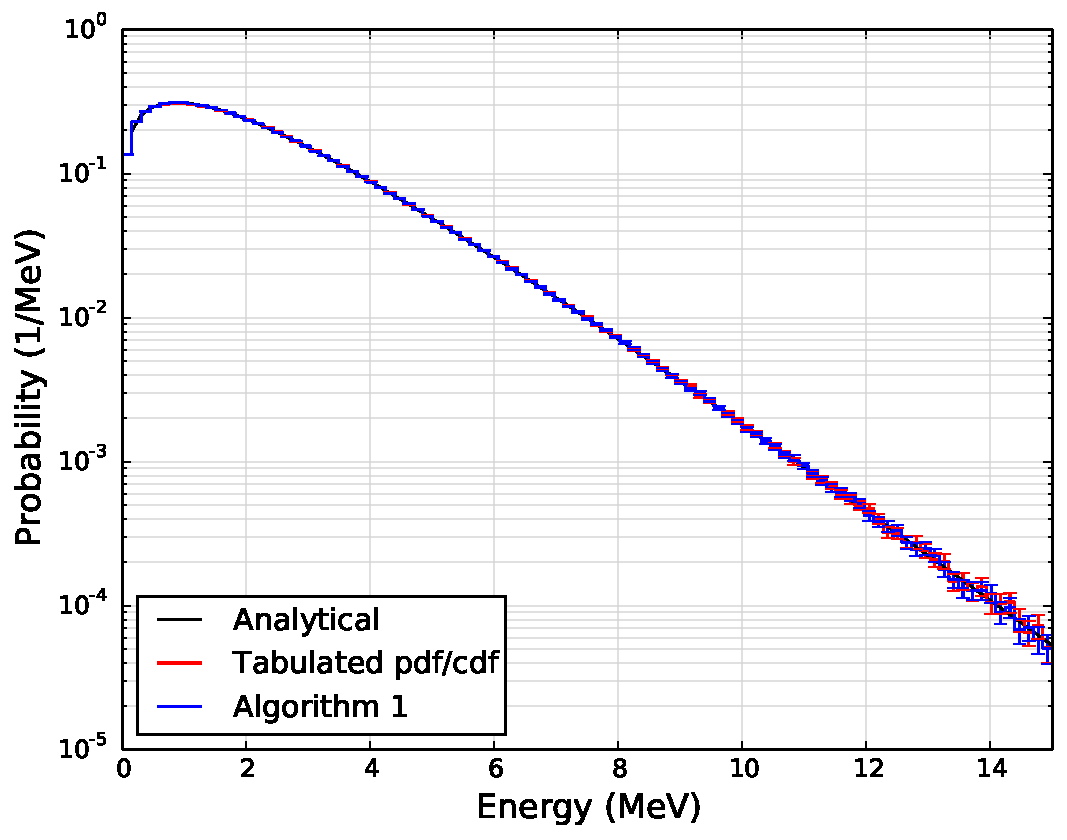
\includegraphics[width=3.0in]{images/spectrum-point-semilogy.pdf}
    \caption{High-energy tail}
  \end{subfigure}
  ~
  \begin{subfigure}[t]{0.45\textwidth}
    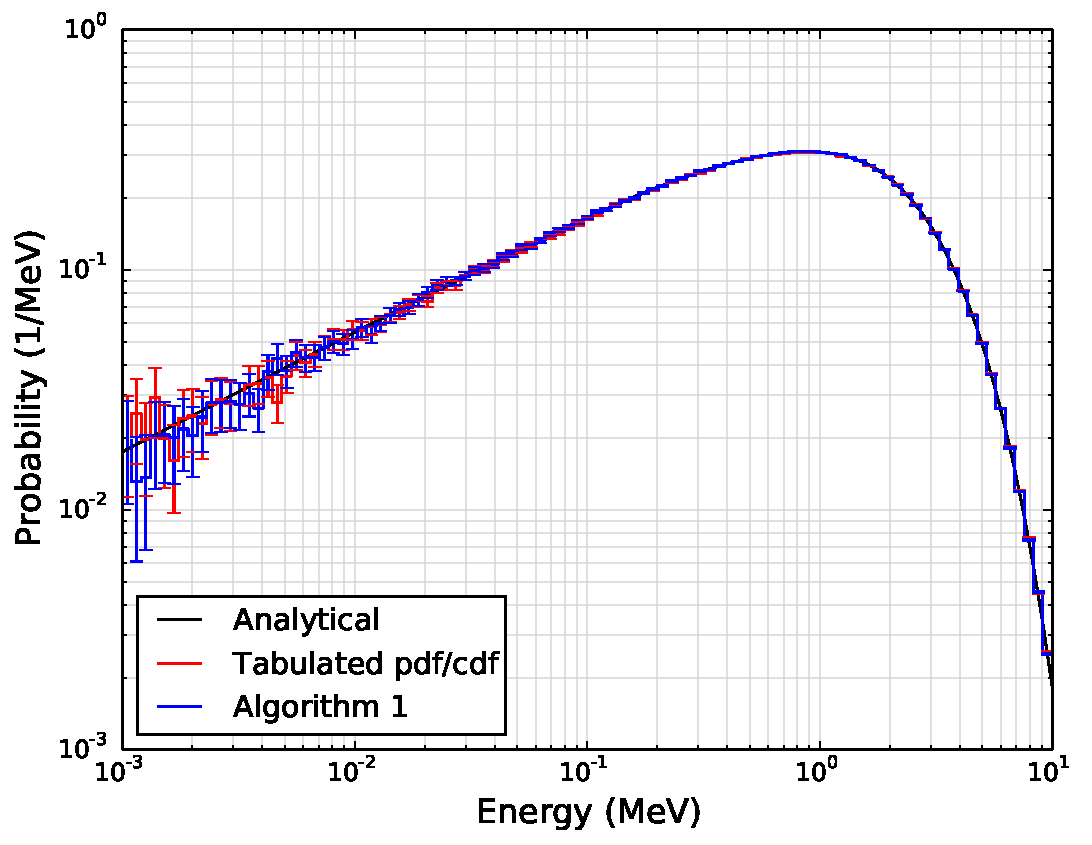
\includegraphics[width=3.0in]{images/spectrum-point-loglog.pdf}
    \caption{Low-energy tail}
  \end{subfigure}
  \caption{Distribution of random variates for the $^{241}$Am fission spectrum
    at $\SI{1e-5}{\electronvolt}$ generated using \autoref{alg:madland-nix} and
    the traditional algorithm compared to \autoref{eq:spectrum}. Error bars
    represent the $2\sigma$ uncertainty.}
  \label{fig:point}
\end{figure}


The second energy, $\SI{0.02}{\electronvolt}$, was chosen to correspond to an
incident energy between values at which $\tmax$ was tabulated, implying that
the traditional algorithm may not be exact. \autoref{fig:between} shows the
observed distribution of 10 million variates produced by each algorithm
compared to the analytical form in \autoref{eq:spectrum}. Again, both
algorithms are shown to be very accurate in the low-energy and high-energy
tails.
\begin{figure}[H]
  \centering
  \begin{subfigure}[t]{0.45\textwidth}
    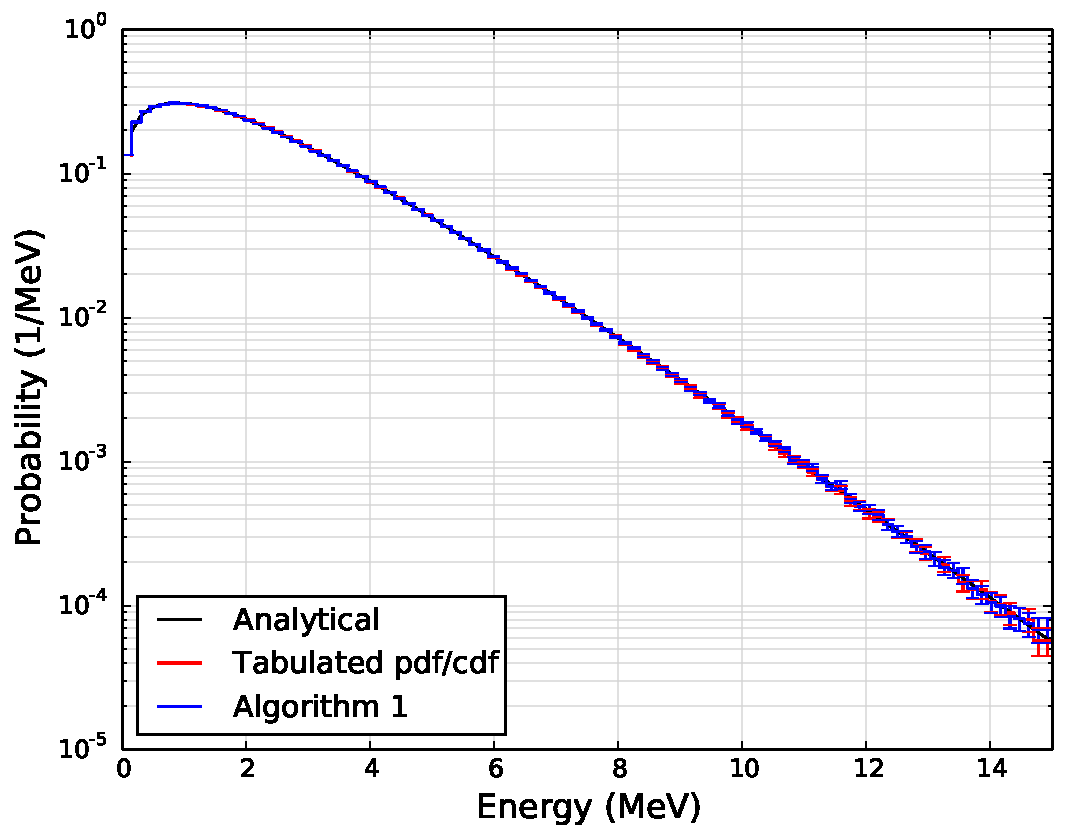
\includegraphics[width=3.0in]{images/spectrum-between-semilogy.pdf}
    \caption{High-energy tail}
  \end{subfigure}
  ~
  \begin{subfigure}[t]{0.45\textwidth}
    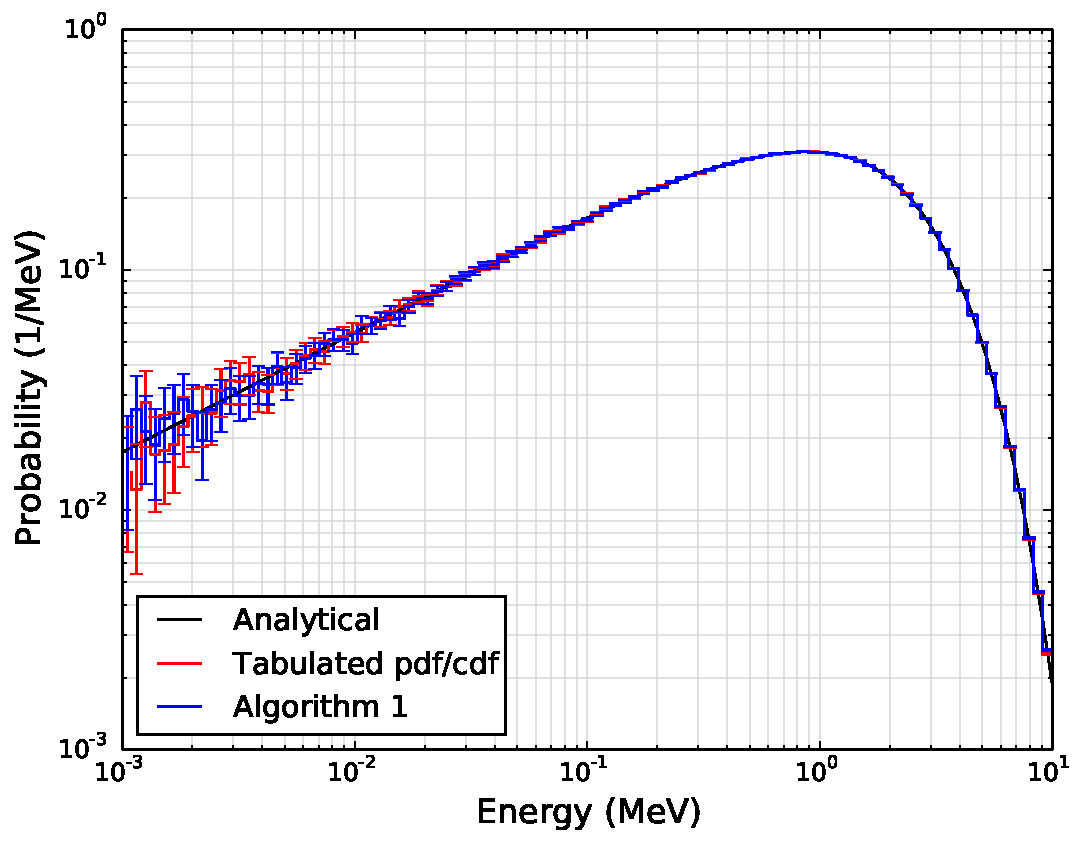
\includegraphics[width=3.0in]{images/spectrum-between-loglog.pdf}
    \caption{Low-energy tail}
  \end{subfigure}
  \caption{Distribution of random variates for the $^{241}$Am fission spectrum
    at $\SI{0.02}{\electronvolt}$ generated using \autoref{alg:madland-nix} and
    the traditional algorithm compared to \autoref{eq:spectrum}. Error bars
    represent the $2\sigma$ uncertainty.}
  \label{fig:between}
\end{figure}

In terms of speed, \autoref{alg:madland-nix} was found to be slightly faster
than the traditional algorithm for the cases being tested. To generate 10
million variates, the traditional algorithm took \SI{0.83}{\second} compared to
\SI{0.57}{\second} for \autoref{alg:madland-nix}. There is also a substantial
savings in memory space; for the ENDF/B-VII.1 $^{241}$Am fission spectrum,
\autoref{alg:madland-nix} needs \SI{904}{\byte} of data for all incoming
neutron energies whereas the traditional algorithm requires
\SI{79.4}{\kilo\byte}.

%%%%%%%%%%%%%%%%%%%%%%%%%%%%%%%%%%%%%%%%%%%%%%%%%%%%%%%%%%%%%%%%%%%%%%%%%%%%%%%%
\section{Conclusions}

By going through a derivation of the probability density function for the
Madland-Nix spectrum, it was shown that an algorithm could be devised to
generate random variates for the spectrum based on physics considerations. This
algorithm can be used by Monte Carlo particle transport codes to sample
secondary energy distributions for fission that are represented using the
Madland-Nix distribution, and only the parameters $\tmax$, $\efl$, and $\efh$
need to be stored in memory. Furthermore, if Monte Carlo codes can use the
parameters directly to sample the Madland-Nix spectrum, nuclear data processing
codes do not need convert the source data from an ENDF-6 format evaluation into
a tabulated probability distribution. Lastly, a Julia program was written to
generate random variates using the algorithm developed herein as well as a
traditional search on the tabulated cumulative density function. A comparison
of the algorithms showed that both are accurate when compared to the analytical
form of the probability density function while the newly developed algorithm is
slightly faster for the cases examined.

%%%%%%%%%%%%%%%%%%%%%%%%%%%%%%%%%%%%%%%%%%%%%%%%%%%%%%%%%%%%%%%%%%%%%%%%%%%%%%%%
\section*{References}

\bibliographystyle{elsarticle-num}
\bibliography{references}

\end{document}
